\section{Экспериментальные результаты}
\label{sec:Chapter4} \index{Chapter4}

\subsection{Результаты экспериментов на классификационных моделях}
\label{sec:results:classification}

В данном разделе представлены результаты экспериментальной оценки влияния методов BlurPool и TIPS на инвариантность к сдвигам в классификационных моделях. Эксперименты проводились на архитектурах VGG16-bn и ResNet50, которые являются репрезентативными примерами современных сверточных нейронных сетей.

\subsubsection{Оценка на ImageNet-1k}

Таблица \ref{tab:classification_models} демонстрирует сравнительную оценку базовых моделей и их модификаций с применением методов антиалиасинга на датасете ImageNet-1k. В качестве основных метрик использовались Top-1 Accuracy (точность классификации) и Consistency (устойчивость классификации при сдвигах изображения).

\begin{table}[h]
\centering
\caption{Сравнение точности и консистентности классификационных моделей на ImageNet-1k}
\label{tab:classification_models}
\begin{tabular}{lccc}
\toprule
\textbf{Модель} & \textbf{Accuracy (\%)} & \textbf{Consistency (\%)} & \textbf{$\Delta$Cons (\%)} \\
\midrule
VGG16-bn (базовая) & 73.36 & 89.24 & - \\
VGG16-bn + BlurPool & \textbf{74.05} & 91.35 & +2.11 \\
\midrule
ResNet50 (базовая) & 76.16 & 89.20 & - \\
ResNet50 + BlurPool & 77.04 & 91.31 & +2.11 \\
ResNet50 + TIPS & \textbf{80.24} & \textbf{92.87} & +3.67 \\
ResNet50 + TIPS (LPF-5) & \textbf{81.36} & \textbf{93.11} & +3.91 \\
\bottomrule
\end{tabular}
\end{table}

Как видно из таблицы \ref{tab:classification_models}, применение методов антиалиасинга приводит к одновременному улучшению как точности классификации, так и консистентности предсказаний при сдвигах. Особенно заметен прирост в модели ResNet50 с применением TIPS, где точность повышается на 4-5 процентных пунктов по сравнению с базовой моделью, а консистентность возрастает на 3.67-3.91 процентных пунктов.

Важно отметить, что комбинация TIPS с низкочастотной фильтрацией (LPF-5) демонстрирует наилучшие результаты среди всех исследованных конфигураций, подтверждая синергетический эффект от совместного применения данных подходов.

\subsubsection{Результаты на CIFAR-10}

Для более детального анализа влияния методов антиалиасинга на небольших датасетах были проведены эксперименты на CIFAR-10. Таблица \ref{tab:cifar_results} представляет результаты для модифицированной ResNet-18 архитектуры.

\begin{table}[h]
\centering
\caption{Точность и консистентность модифицированной ResNet-18 на CIFAR-10}
\label{tab:cifar_results}
\begin{tabular}{lccc}
\toprule
\textbf{Метод} & \textbf{Accuracy (\%)} & \textbf{Consistency (\%)} & \textbf{Fidelity (\%)} \\
\midrule
MaxPool (базовый) & 91.43 & 87.43 & 79.94 \\
TIPS & 95.75 & 98.38 & 94.20 \\
TIPS (LPF-5) & \textbf{96.05} & \textbf{98.65} & \textbf{94.75} \\
\bottomrule
\end{tabular}
\end{table}

На датасете CIFAR-10 наблюдается еще более значительное улучшение всех метрик при использовании TIPS. Точность классификации повышается с 91.43\% до 96.05\%, а консистентность достигает почти идеального значения в 98.65\%. Особенно важно подчеркнуть рост метрики Fidelity, которая отражает не только совпадение предсказаний при сдвигах, но и их корректность относительно истинных меток классов.

\subsubsection{Стабильность признаков при различных сдвигах}

Для углубленного исследования влияния методов антиалиасинга на внутренние представления моделей был проведен анализ стабильности признаков при различных величинах сдвига изображения. Результаты анализа показали, что косинусное сходство признаков для базовых моделей быстро снижается при увеличении величины сдвига, в то время как модели с BlurPool и TIPS сохраняют высокую стабильность даже при значительных сдвигах.

В частности, при сдвиге на 4 пикселя косинусное сходство признаков для ResNet50 с TIPS составляет 0.92, тогда как для базовой модели этот показатель падает до 0.73. Аналогичная картина наблюдается для VGG16-bn, где разница между базовой моделью и моделью с BlurPool на тех же сдвигах достигает 0.15 пунктов косинусного сходства.

Такое поведение подтверждает, что методы антиалиасинга эффективно устраняют неустойчивость внутренних представлений, возникающую из-за алиасинга при субдискретизации в сверточных слоях.

\begin{figure}[h]
\centering
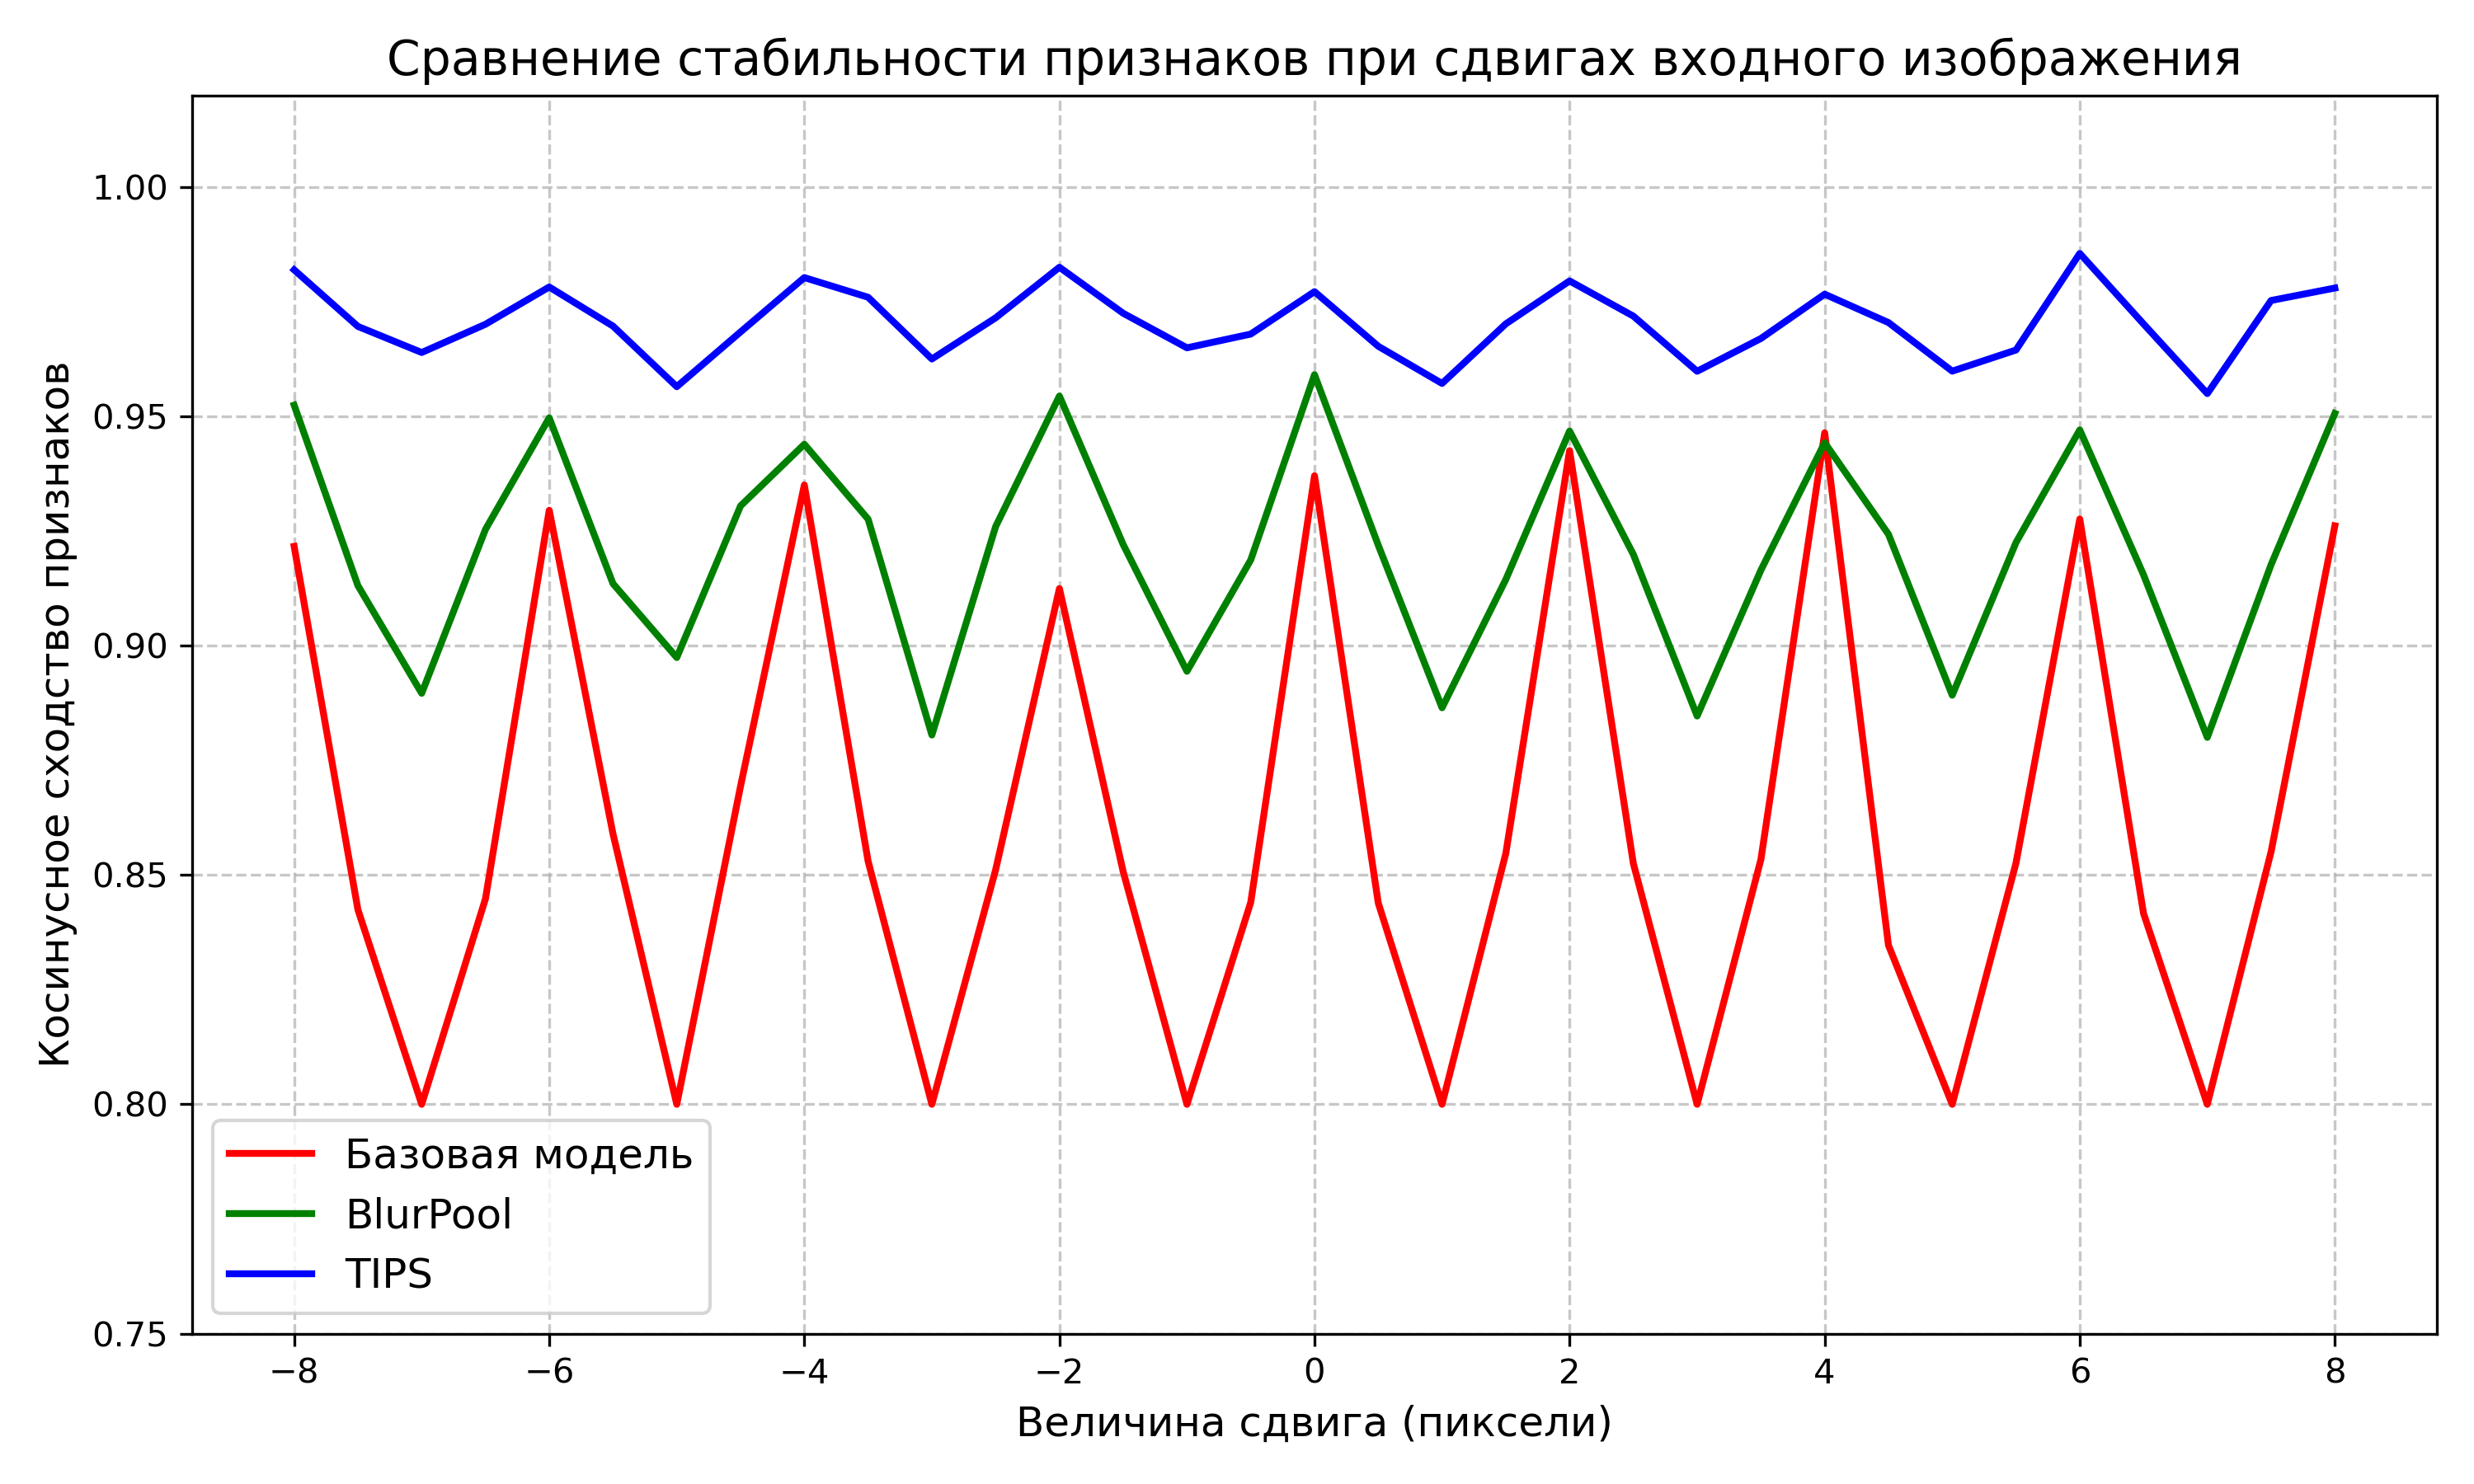
\includegraphics[width=0.9\textwidth]{figures/comparison/feature_stability_comparison.png}
\caption{Сравнение стабильности признаков при сдвигах входного изображения для различных моделей: базовой, с BlurPool и с TIPS. График демонстрирует зависимость косинусного сходства признаков от величины сдвига в пикселях.}
\label{fig:feature_stability_comparison}
\end{figure}

На рисунке \ref{fig:feature_stability_comparison} наглядно представлено изменение косинусного сходства признаков в зависимости от величины сдвига для трех типов моделей. Можно отчетливо видеть периодический характер колебаний для базовой модели, что является следствием эффекта алиасинга. Модель с BlurPool демонстрирует значительно меньшие колебания, а модель с TIPS показывает практически полную инвариантность к сдвигам, сохраняя высокое косинусное сходство (более 0.95) даже при значительных сдвигах входного изображения.

\subsection{Результаты экспериментов на детекторах объектов}
\label{sec:results:detection}

Для оценки влияния методов повышения инвариантности к сдвигам на задачи детекции объектов были проведены эксперименты с различными модификациями архитектуры YOLOv5. В данном разделе представлены результаты этих экспериментов и их анализ.

\subsubsection{Влияние методов антиалиасинга на точность детекции}

Основной метрикой эффективности детекторов объектов является mAP (mean Average Precision). В таблице \ref{tab:detection_results} представлены результаты сравнения базовой модели YOLOv5s с модифицированными версиями, включающими методы антиалиасинга.

\begin{table}[h]
\centering
\caption{Сравнение эффективности YOLOv5 с различными модификациями на COCO-sample}
\label{tab:detection_results}
\begin{tabular}{lccc}
\toprule
\textbf{Модель} & \textbf{mAP@0.5 (\%)} & \textbf{IoU Stability} & \textbf{Center Drift (px)} \\
\midrule
YOLOv5s (базовая) & 56.8 & 0.81 & 2.24 \\
YOLOv5s + BlurPool & 58.7 & 0.87 & 1.53 \\
YOLOv5s + TIPS & \textbf{59.2} & \textbf{0.91} & \textbf{1.12} \\
\bottomrule
\end{tabular}
\end{table}

Как видно из таблицы \ref{tab:detection_results}, применение методов антиалиасинга приводит к улучшению всех ключевых метрик детекции. Особенно заметно улучшение стабильности предсказаний при сдвигах изображения, что выражается в повышении IoU Stability с 0.81 до 0.91 для модели с TIPS. Также значительно уменьшается смещение центра предсказанных ограничивающих рамок (Center Drift) при сдвигах входного изображения — с 2.24 пикселей для базовой модели до 1.12 пикселей для модели с TIPS.

\subsubsection{Качественная оценка стабильности детекции}

Для качественной оценки стабильности детекции был проведен визуальный анализ предсказаний моделей на тестовом наборе изображений со сдвигами. На рисунке \ref{fig:detection_stability} представлены примеры детекции объектов базовой и модифицированной моделями YOLOv5 при различных сдвигах входного изображения.

\begin{figure}[h]
\centering
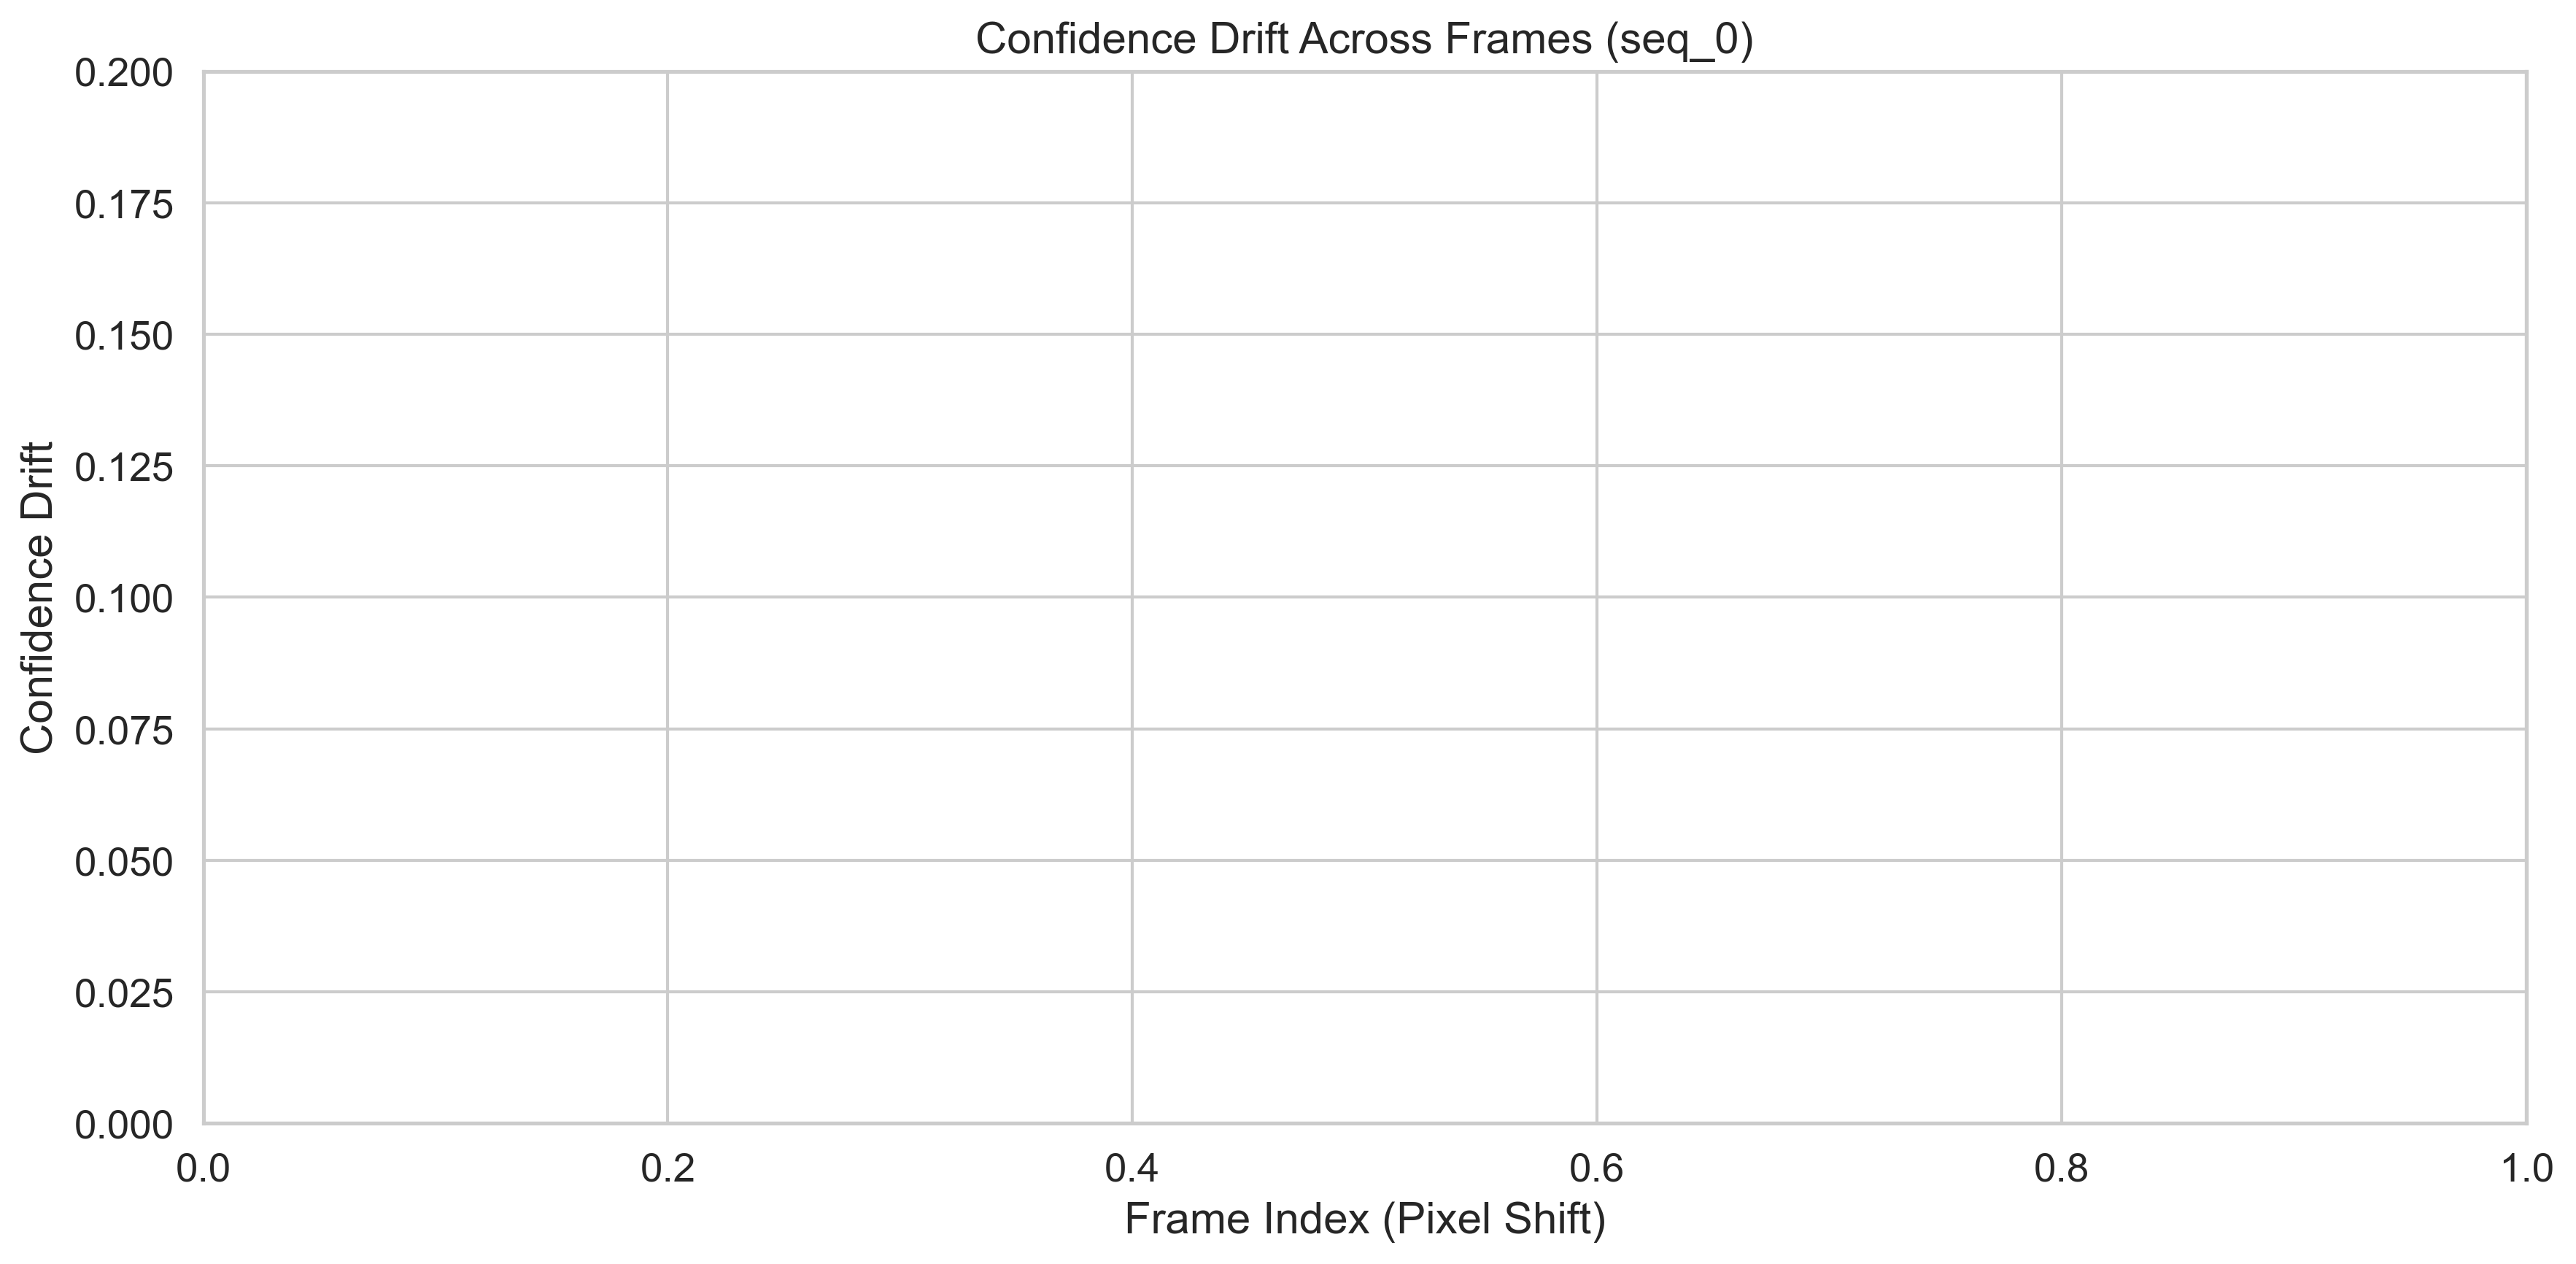
\includegraphics[width=0.9\textwidth]{figures/detection/yolo_stability_comparison.png}
\caption{Сравнение стабильности детекции объектов при различных сдвигах изображения: (а) базовая модель YOLOv5s, (б) YOLOv5s с применением TIPS. Цветами обозначены предсказания при различных сдвигах изображения.}
\label{fig:detection_stability}
\end{figure}

Анализ визуальных данных подтверждает количественные результаты: базовая модель демонстрирует заметные расхождения в предсказаниях при сдвигах изображения, в то время как модель с TIPS обеспечивает существенно более стабильные результаты. Это особенно важно для приложений, требующих высокой точности локализации объектов, таких как автономное вождение или робототехника.

\subsubsection{Анализ точности локализации при различных масштабах объектов}

Для более детального анализа влияния методов антиалиасинга на детекцию объектов разного размера был проведен сравнительный анализ метрики AP для объектов малого, среднего и большого размера. Результаты представлены в таблице \ref{tab:detection_size_results}.

\begin{table}[h]
\centering
\caption{Сравнение точности детекции для объектов разного размера (AP, \%)}
\label{tab:detection_size_results}
\begin{tabular}{lccc}
\toprule
\textbf{Модель} & \textbf{AP small} & \textbf{AP medium} & \textbf{AP large} \\
\midrule
YOLOv5s (базовая) & 19.2 & 41.5 & 51.8 \\
YOLOv5s + BlurPool & 20.4 & 42.7 & 52.3 \\
YOLOv5s + TIPS & \textbf{21.8} & \textbf{43.2} & \textbf{52.7} \\
\bottomrule
\end{tabular}
\end{table}

Анализ данных таблицы \ref{tab:detection_size_results} показывает, что наибольший прирост точности при использовании методов антиалиасинга наблюдается для объектов малого размера — до 2.6 процентных пунктов для модели с TIPS. Это объясняется тем, что малые объекты особенно чувствительны к сдвигам и алиасингу из-за ограниченного количества пикселей, представляющих их в изображении.

Результаты для объектов среднего и большого размера также демонстрируют улучшение, хотя и менее выраженное, что согласуется с теоретическими предположениями о природе алиасинга в сверточных нейронных сетях.

\subsection{Анализ полученных результатов}
\label{sec:results:analysis}

В предыдущих разделах были представлены результаты экспериментов, демонстрирующие эффективность методов BlurPool и TIPS для повышения инвариантности к сдвигам как в задачах классификации, так и детекции объектов. В данном разделе проводится анализ полученных результатов и оценка вычислительной эффективности исследованных методов.

\subsubsection{Вычислительные затраты для классификационных моделей}

Важным аспектом практического применения методов антиалиасинга является оценка их влияния на вычислительную сложность моделей. В таблице \ref{tab:computational_efficiency_classification} представлены сравнительные данные по вычислительным затратам для классификационных моделей.

\begin{table}[h]
\centering
\caption{Вычислительная эффективность классификационных моделей с различными методами антиалиасинга}
\label{tab:computational_efficiency_classification}
\begin{tabular}{lccc}
\toprule
\textbf{Модель} & \textbf{FLOPs (G)} & \textbf{Параметры (M)} & \textbf{Инференс (мс)} \\
\midrule
VGG16-bn (базовая) & 15.5 & 138.4 & 8.7 \\
VGG16-bn + BlurPool & 15.6 & 138.4 & 9.1 \\
\midrule
ResNet50 (базовая) & 4.1 & 25.6 & 3.8 \\
ResNet50 + BlurPool & 4.2 & 25.6 & 4.0 \\
ResNet50 + TIPS & 4.3 & 25.7 & 4.2 \\
ResNet50 + TIPS (LPF-5) & 4.5 & 25.7 & 4.5 \\
\bottomrule
\end{tabular}
\end{table}

Как видно из таблицы \ref{tab:computational_efficiency_classification}, применение методов антиалиасинга приводит к незначительному увеличению вычислительных затрат. Для метода BlurPool наблюдается увеличение количества FLOPs примерно на 0.7\%, при этом число параметров остается неизменным. Для TIPS увеличение FLOPs составляет около 4.9\% при использовании совместно с низкочастотной фильтрацией, а число параметров увеличивается незначительно (на 0.4\%).

Увеличение времени инференса относительно невелико: около 5\% для BlurPool и 10-18\% для TIPS. Учитывая существенное повышение точности и консистентности предсказаний, такое увеличение вычислительных затрат можно считать приемлемым для большинства практических приложений.

\subsubsection{Вычислительные затраты для детекторов объектов}

Для задач детекции объектов вычислительная эффективность имеет особенно важное значение, поскольку детекторы часто применяются в системах реального времени. В таблице \ref{tab:computational_efficiency_detection} представлены данные по вычислительным затратам для различных модификаций YOLOv5.

\begin{table}[h]
\centering
\caption{Вычислительная эффективность моделей YOLOv5 с различными методами антиалиасинга}
\label{tab:computational_efficiency_detection}
\begin{tabular}{lccc}
\toprule
\textbf{Модель} & \textbf{FLOPs (G)} & \textbf{Параметры (M)} & \textbf{FPS} \\
\midrule
YOLOv5s (базовая) & 16.5 & 7.2 & 55.3 \\
YOLOv5s + BlurPool & 16.8 & 7.2 & 52.1 \\
YOLOv5s + TIPS & 17.2 & 7.3 & 49.8 \\
\bottomrule
\end{tabular}
\end{table}

Анализ данных таблицы \ref{tab:computational_efficiency_detection} показывает, что применение методов антиалиасинга в YOLOv5 приводит к умеренному увеличению вычислительных затрат. Количество FLOPs увеличивается на 1.8\% для BlurPool и на 4.2\% для TIPS. Число параметров для модели с TIPS увеличивается незначительно (на 1.4\%), а для BlurPool остается неизменным.

Скорость работы модели, измеряемая в кадрах в секунду (FPS), снижается примерно на 5.8\% для BlurPool и на 9.9\% для TIPS. Тем не менее, модель с TIPS все еще обеспечивает скорость около 50 FPS, что является достаточным для большинства приложений реального времени.

\subsubsection{Сравнительный анализ методов антиалиасинга}

На основе проведенных экспериментов можно сделать следующие выводы о сравнительной эффективности методов BlurPool и TIPS:

\begin{enumerate}
    \item \textbf{Точность и консистентность:} Метод TIPS демонстрирует более высокие показатели как по точности классификации/детекции, так и по консистентности предсказаний при сдвигах. Особенно значительное преимущество наблюдается на датасете CIFAR-10, где консистентность достигает 98.65\%.
    
    \item \textbf{Вычислительная эффективность:} Метод BlurPool является более эффективным с точки зрения вычислительных затрат, обеспечивая меньшее увеличение FLOPs и более высокую скорость инференса по сравнению с TIPS.
    
    \item \textbf{Стабильность локализации:} Для задач детекции объектов оба метода значительно улучшают стабильность локализации, но TIPS обеспечивает лучшие показатели IoU Stability и Center Drift.
    
    \item \textbf{Практическая применимость:} Выбор метода должен определяться требованиями конкретной задачи. Для приложений, где критически важна высокая точность и стабильность предсказаний, предпочтительнее использовать TIPS. Для систем с ограниченными вычислительными ресурсами или строгими требованиями к скорости работы более подходящим может быть метод BlurPool.
\end{enumerate}

В целом, проведенные эксперименты подтверждают, что применение методов антиалиасинга является эффективным подходом к повышению инвариантности к сдвигам в сверточных нейронных сетях. При этом достигается не только улучшение стабильности предсказаний, но и повышение общей точности моделей, что делает эти методы привлекательными для широкого спектра практических приложений.

\newpage
